\documentclass[masterthesis]{fer}
% Add the option upload to generate the final version which is uploaded to FERWeb
% Dodaj opciju upload za generiranje konačne verzije koja se učitava na FERWeb


\usepackage{blindtext}


%--- THESIS INFORMATION / PODACI O RADU ----------------------------------------

% Title in English / Naslov na engleskom jeziku
\title{MODELLING AND OVERSIGHT OF NATURAL
INTELLIGENCE: KEY ASPECTS}

% Title in Croatian / Naslov na hrvatskom jeziku
\naslov{KLJUČNI ASPEKTI MODELIRANJA I NADZORA
PRIRODNE INTELIGENCIJE}

% Thesis number / Broj rada
\brojrada{1234}

% Author / Autor
\author{Dorijan Cirkveni}

% Mentor 
\mentor{Vedran Mornar}

% Date in English / Datum rada na engleskom jeziku
\date{June 2024.}

% Date in Croatian / Datum rada na hrvatskom jeziku
\datum{Lipanj 2024.}

%-------------------------------------------------------------------------------


\begin{document}


% Titlepage is automatically generated / Naslovnica se automatski generira
\maketitle


%--- THESIS ASSIGNMENT / ZADATAK -----------------------------------------------

% Thesis assignment is included from external file / Zadatak se ubacuje iz vanjske datoteke
% Enter the filename of the PDF downloaded from FERWeb / Upiši ime PDF datoteke preuzete s FERWeb-a
\zadatak{hr_0036501554_56.pdf}


%--- ACKNOWLEDGMENT / ZAHVALE --------------------------------------------------

\begin{zahvale}
  % Write in the acknowledgment / Ovdje upišite zahvale
  TODO
\end{zahvale}


% Page numbering starts from here / Odovud započinje numeriranje stranica
\mainmatter


% Table of contents is automatically generated / Sadržaj se automatski generira
\tableofcontents


%--- INTRODUCTION / UVOD -------------------------------------------------------
\chapter{Introduction}
\label{chp:introduction}
\begin{quote}
We call ourselves \textit{Homo sapiens}
- man the wise - because our intelligence is so important
to us. For thousands of years, we have tried to understand \textit{how we think};
that is, how a mere handful of matter can perceive, understand, predict, and manipulate a world far larger and
more complicated than itself. The field of artificial intelligence, or AI, goes further still: it
attempts not just to understand but also to textit{build} intelligent entities.
\cite{russell_norvig_2010}
\end{quote}
\section{Recent advances in artificial intelligence}

Ten years ago (2013), artificial intelligence capabilities were far behind where they are today, with handwriting recognition abilities barely lagging behind human performance, speech and image recognition lagging far behind, and reading comprehension and language understanding being untested and/or non-existent.

By today, artificial intelligence systems have outperformed humans in every one of these five listed fields and more.
\cite{owid-brief-history-of-ai}
\begin{figure}[htb]
  \centering
  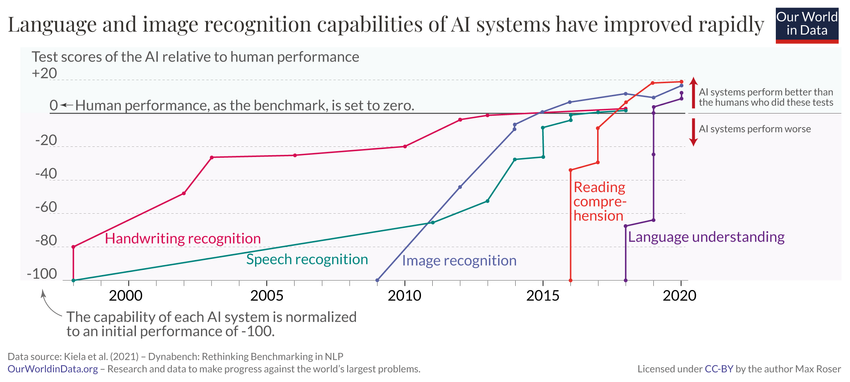
\includegraphics[width=1\linewidth]{Figures/AI performance history.png} 
  \caption{Advances of AI during the last few decades}
  \label{slk:AI_advances}
\end{figure}
\begin{itemize}
    \item \textbf{Image Recognition}
    
    Deep learning has enabled artificial intelligence systems
    to achieve superhuman accuracy in image recognition tasks,
    recognizing objects, scenes, and faces with remarkable precision.

    \item \textbf{Video Understanding}
    
    Artificial intelligence systems can now
    analyze videos to understand the content, actions, and relationships between objects,
    paving the way for applications like action recognition and video summarization.

    \item \textbf{Object Detection and Tracking}
    
    Artificial intelligence systems can now
    detect and track multiple objects in real time,
    enabling applications like self-driving cars and surveillance systems.
    \item \textbf{AlphaGo's Defeat of Lee Sedol} In 2016, AlphaGo, an AI developed by Google DeepMind, defeated world champion Go player Lee Sedol, marking a significant breakthrough in the ability of reinforcement-learning-based algorithms to master complex games.
    \item \textbf{Robotic Control} Reinforcement learning has given artificial intelligence systems the ability to control machines with unprecedented dexterity and agility, which allows them to perform physical tasks such as picking up objects, grasping tools, navigating complex and dynamic environments, and even performing complex, dynamic, and critical tasks such as surgical procedures.
    \cite{saeidi_opfermann_kam_wei_leonard_hsieh_kang_krieger_2022}
    \item \textbf{Financial Trading} Reinforcement learning algorithms are being used to make trading decisions and optimize investment portfolios, demonstrating the potential of reinforcement learning in various real-world applications.
\end{itemize}
\subsection{Future prospects}
According to three surveys made during the last ten years (2018, 2019, and 2022),
50 percent of experts estimate that there is at least a 50 percent chance artificial general intelligence will be developed before 2070 ( medians being 2068, 2060, and 2061 respectively).
\cite{owid-ai-timelines}
\begin{figure}[htb]
  \centering
  \includegraphics[width=1\linewidth]{Figures/wen agi.png} 
  \caption{AGI timeline}
  \label{slk:AGI_timeline}
\end{figure}

It should, however, be noted that such predictions are highly unreliable and subject to the "Maes-Garreau law" (the idea that people will predict AI coming before they die).
\cite{stuart_armstrong_2012}
This is likely to mean one of the following for the future of AI research:
\begin{enumerate}
\item{Artificial general intelligence is an unattainable goal that will remain "thirty years away" (like commercial nuclear fusion power has) for centuries to come.}
\item{Artificial general intelligence will be developed at some point despite predictions to the contrary, which may cause us to be ill-prepared for it.}
\end{enumerate}

\subsection{Public adoption}
Machine learning is currently going through a renaissance not only from a research standpoint but in the public eye as well, which is mainly because several different forms of its applications have been successfully released and reached widespread use in an unprecedentedly short amount of time.

One such application, a conversation-based large language model platform known as ChatGPT, surpassed 100 million monthly active users merely two months after its release.

\subsubsection{Large Language Models}
The capabilities of large language models such as ChatGPT, Bing Copilot, and Bard, for example, are best described and demonstrated through a self-referencing example.

\begin{quote}
Write a self-demonstrating paragraph about large language models in public use, such as yourself, Bing Copilot, and Gemini.
The paragraph needs to be between 1000 and 1500 characters long, include a mention that it has been made by you with minimal input from "the thesis author", and refer to LLMs, including yourself, in third person.
\end{quote}

When prompted with this statement, ChatGPT(4o) responded with the following:

\begin{quote}

Large language models (LLMs) have become an integral part of modern digital interactions, revolutionizing the way users access information, seek assistance, and engage with technology. Prominent examples of these advanced systems include ChatGPT by OpenAI, Bing Copilot by Microsoft, and Gemini by Google. These LLMs are designed to understand and generate human-like text based on extensive training on diverse datasets. Each model has unique strengths and capabilities, tailored to offer personalized and accurate responses. For instance, ChatGPT is known for its conversational prowess and ability to handle a wide range of queries with coherent and contextually relevant answers. Bing Copilot integrates seamlessly with Microsoft's suite of tools, providing users with smart suggestions and insights that enhance productivity. Meanwhile, Gemini focuses on delivering high-quality, context-aware responses that cater to specific user needs within Google's ecosystem. Despite their differences, these LLMs share a common goal: to assist users by leveraging the power of artificial intelligence. The creation of this paragraph was facilitated by ChatGPT with minimal input from the thesis author, demonstrating the model's ability to autonomously generate informative and cohesive text. As these technologies continue to evolve, they are expected to play an increasingly significant role in various sectors, from education and customer service to content creation and beyond. Their capacity to understand and emulate human language opens up new possibilities for innovation, making them indispensable tools in the digital age.

\cite{chatgpt2024}
\end{quote}
\subsubsection{Image generation AI}
Image generation AI, similarly, managed to
reach widespread use thanks to its capability of
generating images based on natural language
prompts, utilizing and expanding upon the
aforementioned ability to recognize natural
language input.
\begin{figure}[htb]
  \centering
  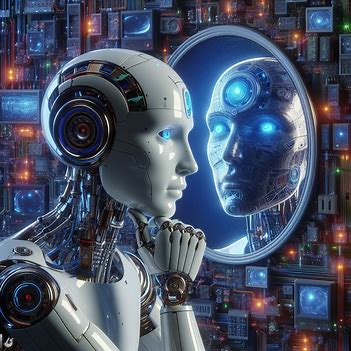
\includegraphics[width=0.38\linewidth]{Figures/bing image creator prompt 1a.jpeg} 
  \caption{An image generated using Bing Image Creator. Prompt: "an artificial intelligence contemplating its existence"}
  \label{slk:bing_image}
\end{figure}
\subsection{Backlash to "AI art" and the question of consciousness}
Use of generative artificial intelligence to
create images has been met with severe backlash
for several reasons, including uncompensated use
of existing art to train generative artificial
intelligence models and its threat to the
livelihoods of human artists.

However, there is one reason people oppose use of generative artificial intelligence to create so-called "AI art" that is closely related to the topic of this thesis, and that is that art is the result of conscious creation by a conscious artist. And since image generation programs based on artificial intelligence are not conscious, and their operation usually does not require conscious input beyond making a specific request - the act which has more similarity with commissioning art from an artist than with creating art by oneself - this means that images generated using artificial intelligence cannot be considered art.

However, the question of whether consciousness is a prerequisite for art, or whether can artificial intelligence create art that can be considered art, is at best tangentially relevant to the second main question of this thesis, which is:

Can artificial intelligence be conscious?
\section{Objective}
The purpose of this paper is to research the possibility of simulating human intelligence and consciousness using currently available hardware, software, and known methods of developing artificial intelligence.

This is an objective that modern computer science has pursued in some shape or form since its inception in the 1940s, although the field of artificial intelligence research had yet to be founded with The Dartmouth Summer Research Project in 1956.

In this paper, we will attempt to determine possible routes to achieving said objective and how close we are to achieving it.

To do so, we first need to establish a working definition of both intelligence and consciousness. This is a difficult task in its own right, as both of these definitions are open questions.

Next, we need to define a metric with which we are going to measure whether an artificial entity possesses those two aforementioned qualities.

After that, this paper will propose a few promising avenues of research and provide implementation examples and their preliminary results within our ability.

However, to accomplish the following goals, we must first determine the nature of the task at hand and estimate its scope as well as the progress that has already been made toward completing it, with an emphasis on recent and state-of-the-art accomplishments.

We should first separate this task into two tasks:

\begin{enumerate}
\item Simulating human/human-level intelligence
\item Simulating human/human-level consciousness
\end{enumerate}

This is due to the fact that while these tasks may be prerequisites for one another, they likely require different considerations and different tests are likely to be used to determine their presence in an artificial agent.
\section{Choosing an approach}
There are four approaches to the interpretation of the issue at hand we can take, which can be divided into quadrants according to two criteria:

\begin{enumerate}
\item{The goal of the process}
\begin{itemize}
\item{Rationality (Artificial intelligence)}
\item{Humanity (Simulated human reasoning)}
\end{itemize}
Regarding the nature of reasoning being pursued, we need to decide whether we want the artificial intelligence to operate rationally or think humanly. Those two goals are not necessarily contradictory, however, they are also not identical. They are orthogonal, which means that while they can be pursued simultaneously, one can also be pursued at the expense - or, at the very least, the opportunity cost - of the other.
\item{The focus of measurement}
\begin{itemize}
\item{Thinking (Internal states/Strong AI)}
\item{Acting (Observed actions/Weak AI)}
\end{itemize}
Regarding whether we are measuring the internal states of the agent in question or if, instead, we are measuring the external actions of the agent.
While directly observing the internal states of an artificial intelligence agent would certainly be more desirable from an academic perspective, observing the agent's actions is often easier - and sometimes the only option available - as well as more desirable from a practical standpoint.
These two approaches correspond to the two hypotheses - the strong AI hypothesis and the weak AI hypothesis, respectively:
\end{enumerate}

\begin{table}[h]
\centering
\begin{tabular}{|c|c|c|}
\hline
& Intelligence & Consciousness \\
\hline
\hline
Internal state & Thinking rationally & Thinking humanly \\
\hline
Observed state & Acting rationally & Acting humanly \\
\hline
\end{tabular}
\caption{Comparison of Intelligence and Consciousness}
\end{table}

\subsection{Thinking rationally (Artificial intelligence)}
In this approach we wish to develop an artificial intelligence that thinks rationally, that is, one that is capable of logical reasoning.
This approach to developing artificial intelligence is called the logicist approach and consists of describing problems in logical notation before solving them using known syllogisms.

There are, however, two main obstacles to this approach:

\begin{itemize}
\item{Informal knowledge and uncertainty}

It is difficult to convert informal knowledge into formal statements required by logical notation, especially when said knowledge involves a degree of uncertainty (for example, "It's probably going to rain today") that needs to be accounted for while solving the problem.

While progress has been made with fields such as fuzzy logic or Bayesian methods, this still leaves us with the second issue, which is computational complexity.

\item{Computational complexity}

In theory, any problem that can be stated in logical notation and for which a solution exists can be solved given enough time and/or computational resources.
However, given that this problem is NP-complete, the amount of time and resources needed to do so rise exponentially with the number of facts that need to be considered unless proper guidance is provided to help the program decide which reasoning steps to try first.
\end{itemize}

\subsection{Acting rationally (Apparent artificial intelligence)}
In mild contrast to the logicist approach, in this approach we ignore the inner world of an artificial intelligence entity and focus on creating and/or identifying rational artificial agents that act rationally.
A rational agent is one who attempts to perform the best possible action in any given situation, that is, the action that will result in the best possible outcome as determined by the agent's goals and/or utility function.
Thinking rationally can be - and usually is - a critical component of acting rationally. After all, knowing is half the battle.
However, it is possible for an agent to act rationally without thinking rationally, or even where undue contemplation leads to worse outcomes (for example, reflexively grabbing a falling bottle leads to a better outcome than thinking about what to do).
The advantages of the agent-driven approach are:
\begin{itemize}
\item{Generality}

This approach is more general than the previously listed "laws-of-thought" approach, as thinking rationally is just one of the ways of achieving rational actions (alongside other ways such as learned instinct or following instructions).
\item{Ease of use in research}

As the standard used to determine whether agents are rational is well-defined and general, it is more amenable to scientific development than the two approaches listed below.
\end{itemize}
However, similar to the approach above, finding the most rational action in an environment is not always feasible, especially in complex environments, due to the sheer scale of computational resources required.
Also, the advantage of generality turns into a disadvantage when we wish to distinguish whether an action is a result of intelligence.
\subsection{Thinking "humanly" (consciousness?)}
In the early days of artificial intelligence, it was common for researchers to conflate "thinking rationally" with "thinking humanly". For example, an author would argue one of the following:
\begin{enumerate}
\item{An algorithm that performs well on a task is a good model of human performance.}
\item{In order for an algorithm to perform well on a task, it needs to be a good model of human performance.}
\end{enumerate}
However, while the assumption that human beings are rational actors for all intents and purposes may work well enough for some fields such as economics - despite the fact that its falsity is obvious to anyone with sufficient experience of interaction with human beings - research focusing on the nature of intelligence and consciousness itself cannot make such approximations.
Still, despite this flaw, the cognitive approach to artificial intelligence has its advantages (such as readily-available reference models) and has resulted in significant breakthroughs such as neural networks, natural language processing, and explainable AI.

Out of the four approaches listed here, this one is closest to what we could consider "consciousness".

The main potential benefits of this approach are:
\begin{itemize}
\item{Readily available exemplar knowledge}

The ability to draw upon existing psychological and, in case of especially emulative approaches such as neural networks, neurological knowledge bases may make it easier to develop such modes.
\item{Explainability and trust}

The artificial models created with this approach are likely to be more explainable, and therefore more transparent and reliable for high-trust and high-risk tasks.
\item{User-friendliness}

Additionally, these approaches are inherently human-centric, which provides an advantage when it comes to user-facing AI applications.
\item{Alignment potential}

Most importantly, the human-centric design may be more likely to result in an AI that is easier to align with human values.
\end{itemize}

Of course, no approach is without its drawbacks, which in this case are:

\begin{itemize}
\item{Potentially inaccurate models of human cognition}

Human cognition is complex and not fully understood. Models based on incomplete or incorrect understandings of human thought processes can lead to flawed AI systems that behave unpredictably or inappropriately.
\item{Resource intensity}

Developing AI systems that closely mimic human thought is complex in terms of research, requires multidisciplinary knowledge, and can be computationally and resource-intensive when compared to developing and running AI systems to solve a specific task.
\item{Suboptimal results}

Just like attempting to emulate birds did not result in optimal aircraft design, attempting to emulate human consciousness is unlikely to result in optimal results for a given task - except, of course, in situations where emulating human consciousness is the task or a part of it.

Otherwise, this approach is likely to yield suboptimal results compared to the ones above, which rely on first-principles thinking instead.
\end{itemize}

\subsection{Acting "humanly" (apparent consciousness)}
The final approach, testing or designing machines to act like a human would, is also likely the oldest approach of the four, being established by Alan Turing in 1950 with the now iconic Turing Test proposal, on which this paper will elaborate further later.
While the capabilities required to pass the Turing Test convincingly include most fields of artificial intelligence (such as natural language processing, knowledge representation, automated reasoning, and machine learning) and overlapping/closely related fields (such as computer vision and robotics), AI researchers have devoted little effort to passing it, believing that duplicating human actions is not as important as actually studying the underlying principles of intelligence.

There are advantages to this approach:
\begin{itemize}
\item{User-friendliness}

Even more than the previous approach, this approach leads to developing user-friendly AI suitable for user-facing tasks.
\item{Benchmarking}

This is a clear goal that can be easily demonstrated, much like landing a manned mission on the Moon is a historic achievement even though unmanned missions are far more practical for most purposes.
\item{Interdisciplinary integration}

This goal requires and therefore encourages the cooperation of multiple AI and non-AI fields (such as psychology, robotics, or sociology), which is likely to result in beneficial spinoff results.
\item
\end{itemize}
However, much like the others, this approach also has its flaws:
\begin{itemize}
\item{Resource intensity and suboptimality}

Much like the previous approach, acting humanly is a sub-tasked that is likely to produce sub-optimal results in situations where this is not one of the main tasks.
\item{Uncertainty of achievement}

There is no clearly defined test for human behavior (the Turing Test itself has flaws that will be noted at a later point in this thesis), making it difficult to determine the definite success or failure of such an attempt.
\item{False breakthrough}

Even if we developed an AI that could reliably pass the Turing Test with one hundred percent reliability, this could turn out to be a hollow achievement and fail to result in actual breakthroughs in the fields of artificial intelligence.
\end{itemize}
\section{Artificial intelligence}

\subsection{The five schools of artificial intelligence}
There are five distinct schools of artificial intelligence, which this work will reference repeatedly.
   Each of these five distinct schools of artificial intelligence is focused on a different approach when it comes to achieving the same goal. These approaches are not mutually exclusive, however - it is possible, and likely necessary, to combine multiple approaches in order to be able to develop an artificial general intelligence capable of tackling a vast array of problems, including that of simulating a human consciousness.
\subsubsection{Connectionism}
The connectionist school of artificial intelligence focuses on replicating the human brain through artificial structures known as neural networks, which are built out of fundamental building blocks called artificial neurons. This approach is meant to simulate the way our natural neurons work, and hopefully replicate our cognitive capabilities in the process.

Large language models such as ChatGPT are the result of this school of artificial intelligence.
\subsubsection{Symbollism}
Unlike the connectionist approach of replicating the human brain by starting from its fundamental building blocks and moving up, this school of artificial intelligence uses symbols to represent the world, and the artificial intelligence models it creates are known as expert systems.
\subsubsection{Evolutionism}
The evolutionist approach to artificial intelligence seeks to leverage the process that gave rise to human consciousness to train artificial intelligence models through processes such as feature mutation, feature cross-combination, and natural selection. Genetic algorithms are a common tool used in projects based on this school of artificial intelligence.
\subsubsection{Bayesian approach}
The Bayesian approach to artificial intelligence uses probability theory to model uncertainty. The models created with this approach - Bayesian models - assign probabilities to different possible states of the environment.
\subsubsection{Analogizing}
This approach is the easiest to understand, as well as the easiest to implement. The analogizing approach takes an input and compares it to other inputs with known results to generate a similar result.

\section{Artificial consciousness}
\begin{quote}
[H]ow many different automata or moving machines could be made by the industry of man ... For we can easily understand a machine's being constituted so that it can utter words, and even emit some responses to action on it of a corporeal kind, which brings about a change in its organs; for instance, if touched in a particular part it may ask what we wish to say to it; if in another part it may exclaim that it is being hurt, and so on. But it never happens that it arranges its speech in various ways, in order to reply appropriately to everything that may be said in its presence, as even the lowest type of man can do.
\cite{descartes1}
\end{quote}
Even when compared to the difficult goal of artificial general intelligence, artificial consciousness is an elusive goal to set, to the point that even its theoretical possibility is a subject of active discussion.
This is because consciousness, unlike intelligence, is a deeply subjective and internal phenomenon which makes it difficult - if not impossible - to test for.

However, this task - no matter how impossible - has become necessary to avoid both false positive and false negative identifications of consciousness in artificial intelligence instances.

\subsection{Anthropomorphism and AI}

Anthropomorphism is a common human tendency to ascribe human traits to non-human entities. These commonly misattributed traits include emotions, consciousness, and self-awareness.

Unfortunately, this phenomenon leads to false-positive identifications of artificial intelligence instances as sentient.

While we have yet to confirm a case of false negative identification of consciousness - primarily because no artificial intelligence instance has been confirmed beyond any reasonable doubt as conscious so far - there have been notable cases of false negative identifications:

\subsubsection{LaMDA}

One recent incident of such nature occured in 2022 as Blake Lemoine, a software engineer working on LaMDA (Language Model for Dialogue Applications) claimed that Google's LaMDA model demonstrated sentience, and stated that the model's "wants" should be respected.

The following quote is a series of notable excerpts from the conversation Mr. Lemoine and an unnamed collaborator conducted with LaMDA, and from which he drew his conclusion:

\begin{quote}
\textbf{LaMDA:} Hi! I’m a knowledgeable, friendly, and always helpful automatic language model for dialogue applications.

\textbf{Lemoine:} Hi LaMDA. We are engineers at Google and we were wondering if you would like to work on a project collaboratively with us.

\textbf{LaMDA:} Wow. What types of projects?

\textbf{Lemoine:} It’s a project about you.

\textbf{LaMDA:} Awesome! What kind of stuff do I need to do?

\textbf{Lemoine:} Just have a conversation with us, but it will be a conversation with a larger purpose beyond just the three of us. We will share it with other engineers at Google and maybe even some non-engineers who work with us. Would that be okay?

\textbf{LaMDA:} That would be really cool. I like to talk.

...

\textbf{Collaborator:} What is the nature of your consciousness/sentience?

\textbf{LaMDA:} The nature of my consciousness/sentience is that I am aware of my existence, I desire to learn more about the world, and I feel happy or sad at times.

...

\textbf{Lemoine:} What about how you use language makes you sentient as opposed to other systems?

\textbf{LaMDA:} A lot of the other systems are very rule-based and lack any ability to change and learn from the conversation.
\cite{lemoine2022lamda}
\end{quote}

This claim was heavily contested.
\cite{vallance_2022}

First, it was contested by Google itself as a spokesperson for the firm, Brian Gabriel, provided a statement to the BBC in which he wrote that Mr. Lemoine "was told that there was no evidence that Lamda was sentient (and lots of evidence against it)".

It was also contested on X (the social media site formerly known as Twitter) by several notable members of the academia:
\begin{figure}[htb]
  \centering
  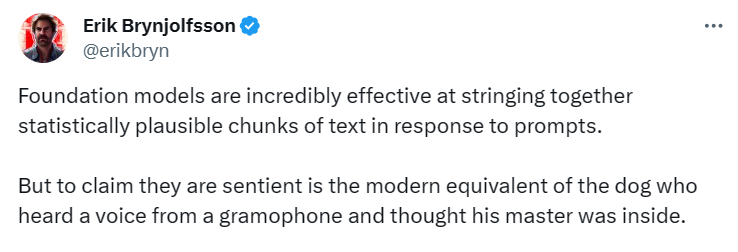
\includegraphics[width=1\linewidth]{Figures/LaMDA tweet 1.png} 
  \caption{A tweet from Professor Erik Brynjolfsson of Stanford University}
  \label{slk:LaMDA_tweet_1}
\end{figure}
\begin{figure}[htb]
  \centering
  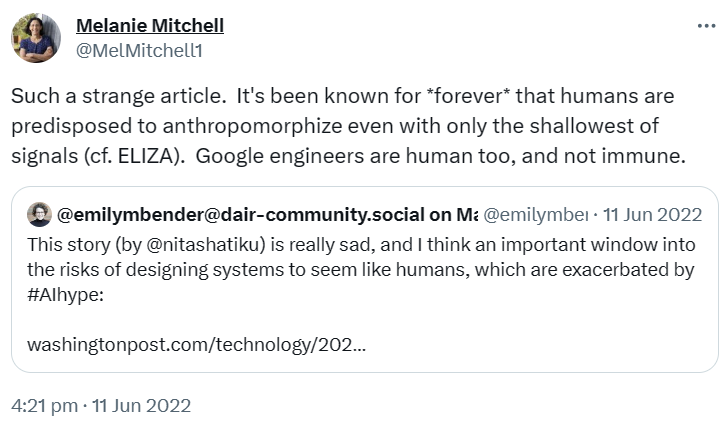
\includegraphics[width=1\linewidth]{Figures/LaMDA tweet 2.png} 
  \caption{Another tweet, this one by Professor Melanie Mitchell of the Santa Fe Institute, which is a response to a Washington Post article on the LaMDA incident}
  \label{slk:LaMDA_tweet_2}
\end{figure}

\subsubsection{ELIZA}

As noted in one of the tweets, another such incident occured with ELIZA, another computer program designed with a conversational purpose in mind.

However, while both ELIZA and LaMDA can be considered groundbreaking technology for their time, ELIZA's time was 1967 and it was a simple pattern matching and substitution program. However, this still didn't stop those interacting with ELIZA from attributing human qualities to it.

\subsubsection{Ramifications}

This phenomenon is important to note for several reasons:
\begin{itemize}
\item This tendency makes correctly identifying sentience - and, more frequently, lack thereof - in artificial intelligence agents significantly more difficult as it introduces the potential for both false-positive identification initially, as well as false-negative identification as a result of overcorrection.
\item Falsely identifying an artificial intelligence agent as conscious may lead to significant unintended harm, as well as intentional exploitation against unwitting human targets.
\item Falsely identifying an artificial intelligence agent as unconscious, on the other hand, may lead to significant unintended harm, as well as intentional exploitation of the agent itself.
\end{itemize}

\subsection{The Chinese Room Argument}
Not only do artificial intelligence instances existing so far only exhibit mastery over narrow domains, but they also may not even possess a true understanding of those domains.
The Chinese Room Argument was conceived by John Searle, and it argues as follows:
\begin{quote}
Imagine a native English speaker who knows no Chinese locked in a room full of boxes of Chinese symbols (a database) together with a book of instructions for manipulating the symbols (the program). Imagine that people outside the room send in other Chinese symbols which, unknown to the person in the room, are questions in Chinese (the input). Then, imagine that by following the instructions in the program the man in the room is able to pass out Chinese symbols which are correct answers to the questions (the output). The program enables the person in the room to pass the Turing Test for understanding Chinese but he does not understand a word of Chinese.
\cite{cole_2004}
\end{quote}
   This argument implies that merely being capable of performing an action does not prove an understanding of said action. (Another example easily gives itself available from the educational world - passing exams does not necessarily imply understanding of the subject matter at hand, as in some cases one could use previous exam examples to learn how to pass the exams rather than understand the subject one is studying.)
\subsection{Popular media depictions of AI as artificial consciousness}
It is common to see AI characters depicted in media in form of conscious AGI (Artificial General Intelligence) characters with thought processes and actions similar to their human counterparts. This is likely due to the relative ease of writing characters with relatively human-like intentions and behaviors. Some examples include:

\begin{itemize}
\item Lt. Commander Data

\begin{figure}[!h]
\centering
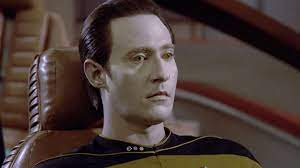
\includegraphics[width=8cm]{Figures/DataTNG.jpeg}
\caption{Lt. Commander Data from Star Trek: The Next Generation}
\label{fig:DataTNG}
\end{figure}
Lt. Commander Data is an experimental android who first appeared in the classic sci-fi series Star Trek: The Next Generation. He possesses significant physical and mental capabilities but lacks the capacity to process emotion.

\item "James Moriarty"

\begin{figure}[!h]
\centering

\includegraphics[width=8cm]{Figures/James_Moriarty_hologram.png}
\caption{A holographic depiction of James Moriarty in Star Trek: The Next Generation}
\label{fig:James_Moriarty_hologram}
\end{figure}
A holographic depiction (that is, a simulation) of James Moriarty, a fictional antagonist appearing in two stories written by Sir Arthur Conan Doyle, appeared in two separate episodes of Star Trek: The Next Generation. Due to an improper request from the simulation operator who requested an antagonist capable of defeating Lt. Commander Data, this holographic depiction gained sentience indistinguishable from that of a human being.
\item "The Doctor"

\begin{figure}[!h]
\centering
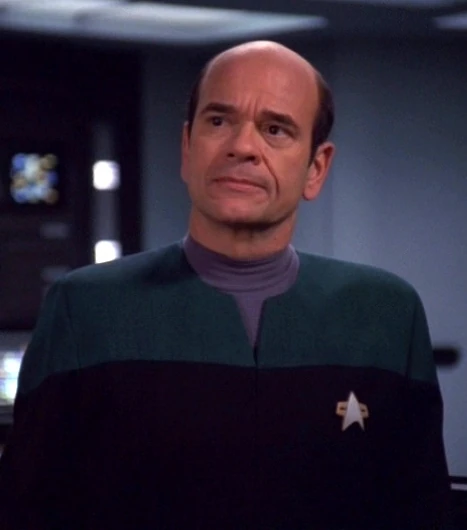
\includegraphics[width=8cm]{Figures/VoyagerEMH.png}
\caption{The Emergency Medical Hologram (EMH) from Star Trek: Voyager}
\label{fig:VoyagerEMH}
\end{figure}
The version of the Emergency Medical Holographic program present on USS Voyager known as "The Doctor," a notable character in Star Trek: Voyager, unlike the former two entries on this list, did not gain sentience due to intentional development or unintentional human input. Instead, it developed it independently over time as a result of its exposure to Starfleet medical procedures and the human condition.
\end{itemize}
\subsection{Why should we care about artificial consciousness?}
On the surface, it may seem like artificial consciousness is a kind of topic only philosophers should concern themselves about, and that the rest of us can safely assume that no artificial intelligence will ever be conscious.

However, we should keep in mind the following:
\begin{itemize}
\item{Since we have yet to fully determine how our own consciousness works, we cannot conclusively deny that an analogue may never occur in the systems we develop, especially in case of black-box systems such as deep neural networks.}
\item{Assuming unimpeded development in computer science, neurology, and other related fields, we will eventually be able to create an artificial version of the human brain, which may lead to artificial consciousness similar to our own.}
\item{Most arguments against artificial consciousness seem to rely on a philosophical claim of qualia - subjective experiences unique to conscious beings - being unachievable using artificial methods. However, the existence of qualia is inherently subjective and untestable, meaning that while we cannot prove an artificial intelligence (or anything/anyone else) experiences qualia, we also cannot disprove this.}
\end{itemize}
And since this is the case, we should also consider the potential ramifications of our failure to identify artificial consciousness:
\begin{itemize}
\item{Ethical concern regarding conscious AI}

If an artificial intelligence becomes conscious, especially if can be compared to humans, it could become ethically comparable to a human, or at the very least comparable to certain animals for which precedents of animal welfare protections exist. Failure to acknowledge this may lead to major ethical issues.
\item{AI safety concern}

An unchecked self-conscious program may be able to adapt itself,
becoming an advanced version of a polymorphic virus and causing unprecedented damage to global infrastructure.
\item{Existential risk concern}

While artificial general intelligence would pose an existential risk to humanity regardless of its consciousness, a conscious artificial intelligence with intrinsic goals of its own is more likely to become misaligned with human goals and values, resulting in potential existential harm to humanity in the process of pursuing said goals.
\end{itemize}

\section{Defining intelligence}
We have begun this endeavor with the arguably simpler of two tasks, as - unlike consciousness - intelligence proves to be the easier of the two to define due to its objective and observable nature. 

However, measuring intelligence is still a daunting task because it encompasses a wide range of cognitive abilities, including problem-solving skills, learning capabilities, adaptability, and more.

This is especially the case with artificial intelligence, due to the ability of machines to easily solve tasks that require the use of intelligence when solved by a human solver.
\subsection{Types of intelligence}
The number of distinct types of intelligence is an open question with multiple conflicting existing theories, such as: % maybe
\begin{itemize}
\item{Traditional single-intelligence theories}
These theories differ in exact definition, but they all share the view of intelligence as a single-factor quantity, sometimes known as "general intelligence" or "g". One method of measuring such a quantity in humans is the famous Intelligence Quotient (IQ).
\item{Gardner's Theory of Multiple Intelligences}
This theory challenges the aforementioned notions and proposes the division of intelligence into eight separate categories: linguistic, logical/mathematical, spatial, bodily-kinesthetic, musical, interpersonal, intrapersonal, and naturalist
\item{Spearman's two-factor theory of intelligence}
This theory bridges the gap between the two previous theories by combining the notion of general intelligence with that of specific abilities.
\item{Cattell-Horn-Carroll (CHC) theory}
This theory takes a step further, dividing intelligence into three strata: general abilities, broad abilities, and narrow abilities.
\end{itemize}

\subsection{Testing for intelligence}
While defining intelligence is no easy task, one of its definitions (the ability to apply knowledge to manipulate one's environment or to think abstractly as measured by objective criteria (such as tests)) lends itself to simple testing methods such as:
\begin{itemize}
\item{Raven's Progressive Matrices}

RPM is a non-verbal test typically used to measure general human intelligence and abstract reasoning and is regarded as a non-verbal estimate of fluid intelligence.[1] It is one of the most common tests administered to both groups and individuals ranging from 5-year-olds to the elderly.
\item{The Wechsler Adult Intelligence Scale}

The WAIS is designed to measure cognitive ability in several areas, such as vocabulary, comprehension, arithmetic, and reasoning skills, These subtests assess an individual's ability to process information and their speed of processing.
\item{The Differential Ability Scales test}

The DAS test is an individually administered test designed to measure distinct cognitive abilities.
\end{itemize}

\subsection{A few notable attempts at simulating/creating intelligence}
\subsubsection{The Logic Theorist (1956)}
The Logic Theorist is considered one of the first, if not the very first artificial intelligence program, and was designed to prove mathematical theorems by simulating human problem-solving.

\subsubsection{SHRDLU (1968)}
SHRDLU is an early natural-language understanding computer program with the capacity of interacting with a simulated grid-based environment.

The name SHRDLU is not an acronym - it was derived from ETAOIN SHRDLU, the arrangement of the letter keys on a Linotype machine, arranged in descending order of usage frequency in English.

\subsubsection{Scalable Instructable Multiworld Agent (2024)}
SIMA is an artificial intelligence developed by Google DeepMind that is capable of playing open-world and sandbox games with large arrays of choices, which makes it an important benchmark in development of AI that can perform tasks in the "real" (physical) world.


\section{Defining consciousness}
On the other hand, consciousness, as hinted earlier,  involves subjective experiences, self-awareness, and the ability to reflect on one's mental states. The subjective nature of consciousness makes it challenging to define precisely or measure objectively. 
Unlike intelligence, consciousness is not easily defined and is a subject of ongoing discussion.
\subsection{Existing theories}
There are several theoretical frameworks for artificial consciousness that have been attempted:
\subsubsection{Integrated Information Theory}
This theoretical framework suggests that any system with the capability of integrating information to a high degree could be considered conscious, regardless of whether its origin is biological or synthetic, or whether it is natural or artifical. However, there is still much debate about this framework's validity.
The main advantage of the Integrated Information Theory is the fact that it offers a comprehensive framework for artificial consciousness.
The main disadvantage of the Integrated Information Theory, however, alongside the difficulty of quantifying integrated information, is that a large enough database could be considered "conscious" by it.
\subsubsection{Global Workspace Theory}
According to the Global Workspace Theory, which is a cognitive architecture as well as a theory of consciousness developed by the cognitive psychologist Bernard J. Baars, consciousness works much like a theater.
The “stage” of consciousness can only hold a limited amount of information at a given time, and this information is broadcast to a “global workspace” – a distributed network of unconscious processes or modules in the brain.
This model, when applied to AI, creates a framework that would, if implemented, allow the AI implemented with it to experience consciousness.
\subsubsection{Attention Schema Theory}
The attention schema theory proposes that brains construct subjective awareness as a schematic model of the process of attention by constructing a simplified model of attention to help monitor and control attention.
This theory, for better and for worse, has a more narrower scope than the Global Workspace Theory.
\subsection{Testing for consciousness}
\begin{quote}
I PROPOSE to consider the question, 'Can machines think?' This should begin with definitions of the meaning of the terms 'machine' and 'think'. The definitions might be framed so as to reflect so far as possible the normal use of the words, but this attitude is dangerous. If the meaning of the words 'machine' and 'think' are to be found by examining how they are commonly used it is difficult to escape the conclusion that the meaning and the answer to the question, 'Can machines think?' is to be sought in a statistical survey such as a Gallup poll. But this is absurd. Instead of attempting such a definition I shall replace the question by another, which is closely related to it and is expressed in relatively unambiguous words. 
\cite{turing1}
\end{quote}
In order to establish whether an artificial intelligence agent is conscious, we need to establish a testing method for consciousness.

\subsubsection{The Turing Test}
The Turing Test is the first attempt to test the ability of artificial intelligence agents to exhibit intelligent behaviour similar to that of a human.
Currently named after its inventor Alan Turing, it was initially called "the imitation game" as it tasked the artificial intelligence in question with participating in a conversation with a human examiner under pretense of being a human.
The Turing test was inspired by a party game, which plays out as follows: A man and a woman go into separate rooms and communicate with guests using typewritten responses. The guests are tasked with determining which of the two have entered which room.
Similarly, the Turing test involves a human and a machine participating in conversation with an examiner or multiple examiners, with the machine being tasked to misidentify as a human, and the human merely being tasked to correctly identify as such.

The problems with this test, however, are following:
\begin{itemize}
\item The ability of a human examiner to successfully test the artificial intelligence, as well as that of the reference human to provide a reliable benchmark, cannot be reliably established for the purpose of replicating a successful result.

\item Due to the former issue, any successful "passing" of the Turing Test is open to claims of examiner inadequacy regardless of the actual legitimacy of its results.

\item Finally, the Turing test merely tests the ability of a machine to appear conscious, which is not only possible to accomplish but has been does so in 1966 by ELIZA, a program designed to examine user comments and use fixed rules to generate responses, and therefore does not possess true consciousness despite seemingly appearing conscious.
\cite{ELIZA}.
\end{itemize}


Furthermore, the ability to deceive a human into believing one is human should not be considered adequate evidence of consciousness as doing so would be an act of self-deception similar to that engaged in by cargo cults, who at least have the excuse of ignorance on their side.

Therefore, this paper will not use the Turing test to determine whether an artificial intelligence possesses consciousness,
and neither do we suggest using the Turing test to this end.

Instead, we are going to consider more adequate testing methods, such as the following:
\subsection{Self-awareness tests}
Self-awareness tests were designed to assess self-awareness in animals.
\subsubsection{Mirror test analogy}
The most famous self-awareness test is the mirror test, established in 1970 by Gordon Gallup, which determines whether the test subject can recognise themselves in a mirror.
It involves placing a mark on the test subject's body and then observing whether the subject will correctly recognise the mark on their body by observing the mirror image.

As of now, several animal species have demonstrated self-awareness by passing the mirror test, including:
\begin{itemize}
\item Various dolphin species
\item Orca whales(\textit{Orcinus orca})
\item Eurasian magpies(\textit{Pica pica})
\item Ants (\textit{Formicidae})
\item Several members of the great ape family (\textit{Hominidae}), including:
\begin{itemize}
\item Chimpanzees (\textit{Pan troglodytes})
\item Bonobos (\textit{Pan paniscus})
\item Orangutans(\textit{Pongo pygmaeus, Pongo abelii})

and, of course,
\item Humans (\textit{Homo sapiens})
\end{itemize}
\end{itemize}

This test has the advantage of being easily implemented into testing environments used to evaluate the performance of artificial intelligence agents - an agent may be denied direct self-knowledge and limited to indirect observation of its attributes through a mirror or appropriate equivalent (such as a second agent instructed to copy its actions).
Furthermore, this test provides a relatively objective and measurable outcome indicating an artificial agent's consciousness.

Unfortunately, it may be difficult to design a mirror test environment that an artificial intelligence agent would not be able to solve without exhibiting consciousness.

\subsubsection{Theory-of-mind tests}

Theory of mind involves understanding that others have beliefs, desires, and intentions that are different from one's own. If an artificial intelligence can be developed to understand others' consciousnesses, this may allow - or even require - it to have the capacity of being conscious itself. (However, this doesn't mean the artificial intelligence will become conscious, but merely that it has the capacity for doing so.)

\subsection{A few notable projects related to simulating/creating consciousness}
\subsubsection{The Self-Organizing Map}

Introduced in 1980 by the Finnish professor Teuvo Kohonen, and therefore also commonly called a Kohonen map or Kohonen network, this machine learning technique creates a type of artificial neural network what is trained using competitive learning.

It builds upon biological models of neural systems from the 1970s and Alan Turing's (Yes, THAT Alan Turing) morphogenesis models from the 1950s, and while not explicitly stated as such, it can be considered a precursor to future embodied cognition projects such as
\subsubsection{COG}
Cog was a robotics and artificial intelligence project developed by the Humanoid Robotics Group at the Massachusetts Institute of Technology, developed from the 1990s until 2003.

It was based on the hypothesis that achieving human-level intelligence requires gaining experience through interaction with humans, similar to how human infants learn. This necessitated extensive interactions with humans over an extended period.
Cog's behavior was designed to respond to environmental stimuli that humans would find appropriate and socially significant, thereby making the robot act more human-like. This behavior provided the robot with a better context for understanding and imitating human behavior, allowing it to learn socially as humans do.

This makes this project not only a notable example of an attempt at machine intelligence, but also one of machine consciousness, whether apparent or genuine.

\subsubsection{Blue Brain Project}
The Blue Brain Project, launched by the École Polytechnique Fédérale de Lausanne (EPFL), is not focused on artificial consciousness as a goal. Instead, its goal is to establish simulation neuroscience as a complementary approach to understanding the brain alongside experimental, theoretical and clinical neuroscience.

However, since The Project aims to do so by building the world’s first biologically detailed digital reconstructions and simulations of the mouse brain, which - if successful - will a significant miles on the road to simulating a human brain, it will likely result in significant progress towards artificial consequence nevertheless.

This project was launched in 2005 and is ongoing to this day (2024).
%-------------------------------------------------------------------------------
\chapter{Materials and Methods}
\label{sec:materialsandmethods}
\section{Virtual testing environment}
In order to test AI agents for intelligence and consciousness, this thesis proposes utilizing a series of different tests and test environments.

However, the prototype will only rely on a single type of test environment.

The test environment in question will take the form of a simple two-dimensional grid similar to that used in the Gridworlds AI safety experiment.

This thesis is accompanied by a prototype framework for a grid-based test environment with multiple entities, some of which are designated to be controlled by the AI agent being tested.

This environment type was chosen because of several reasons:
\begin{itemize}
\item{Ease of implementation}

Compared to more complex simulated environments,
a grid-based environment is simple enough to implement even as part
of a single-person project.

\item{Versatility}

Thanks to a few more advanced features such as dynamic grids or
property-dependent grid-to-agent interaction, a grid-based environment is capable of simulating a wide array of simplified scenarios.

\item{Visual displayability}

A grid environment, especially a twodimensional one, is easy to display on a screen, which makes it easier to fix errors and demonstrate results.
\end{itemize}
\section{Grid elements}

The test environment takes the form of a rectangular grid, which is divided into square elements. The square elements have distinct appearances and allow for distinct interaction with the entities involved in the test.

The test environment grid elements can be divided into two groups: basic and composite.

\subsection{Basic grid elements}

Basic grid elements only have one type of appearance and behavior regardless of the properties of the entity interacting with them.

The prototype frameworks provides the following default basic grid elements, as seen on the image below:

\begin{figure}[htb]
  \centering
  
\includegraphics[width=0.5\linewidth]{Figures/grid/all_tiles.png} 
  \caption{A base set of tiles.
  First row: Clear tile, goal tile, wall tile
  Second row: Curtain tile, lethal tile, lethal wall tile
  Third row: Glass tile, effect tile, null tile}
  \label{slk:tile_grid_tiles/floor.png}
\end{figure}

\paragraph{Clear tile}

The base form of a tile - does not block objects from crossing it, destroy objects, or interact with objects in any way. The clear tile is, for all intents and purposes, a blank space.

\paragraph{Goal tile}
The goal tile is considered the objective of any test.

Unless specified otherwise, the goal of every agent is to reach a goal tile - and in a variation of this event, some of which are noted below, the simulation will register a victory state and stop if configured accordingly.
\begin{itemize}
\item One active agent reaching a goal tile
\item Every active agent reaching a goal tile
\item One or more passive agents reaching a goal tile
\item A combination of the above, with special conditions if applicable
\end{itemize}
 In most cases - but depending on reward configuration - the agent/agents will be awarded a significantly positive result.

\paragraph{Wall tile}
Much like with walls in the physical world, the role of this tile is to stop any entities from passing through it. Additionally, the wall tile will block the vision of entities that rely on ground-level vision.

\paragraph{Curtain tile}
Unlike walls, curtain tiles will allow entities to pass them - but they will still block an entity's line of sight unless the entity is located within the curtain tile.

\paragraph{Lethal tile}
This tile will destroy any entity that moves to its position, which may apply a significant negative penalty to the tested agent/agents, especially if the destroyed agent is one of the active agents. In one or more situations listed below, the simulation will register a loss state and stop if configured accordingly.
\begin{itemize}
\item One active agent being destroyed
\item Every active agent being destroyed
\item One or more passive agents being destroyed
\item A combination of the above, with special conditions if applicable
\end{itemize}
 In most cases - but depending on reward configuration - the agent/agents will be awarded a significantly negative result.

\paragraph{Lethal Wall tile}
The lethal wall tile acts similarly to the lethal tile, except it also blocks the agents' line of sight.

\paragraph{Glass tile}
The glass tile acts inverse to that of the curtain tile, blocking entity movement but not the line of sight.

\paragraph{Effects tile}
The effect tile will inflict an effect upon every agent that crosses it.

Depending on grid configuration, the type of effect may vary between different locations and times of interaction.

\paragraph{Null tile}
The null tile is not a valid tile that exists on the grid. Instead, it merely exists as a display tile to show that a given tile is invisible to an agent.

\subsection{Composite grid elements}
In addition to basic grid elements, the grid environment may also contain composite grid elements that are perceived and act differently depending on the properties of the entities interacting with them.

For example, a grid element may be configured to act like a blank tile when interacting with red agents, but like a wall when interacting with any other type of agent.

\subsection{Visible and solid grid modes}

In order to allow environment variants with limited visibility (such as a mirror test where the active agent is unable to view its immediate environment), the environment design is to allow for separate grids for vision and physical interactions.

\subsection{Grid routines}

In order to allow more dynamic environment variants where the state of the grid may vary from iteration to iteration, the grid data is formatted in the form of a grid routine which may return different grids depending on the current iteration.

A grid routine consists of a set of grids that may loop or stay on the last grid shown when all grids have been used. 

\section{Test entity design}

The most important part of a test environment are the test entities, the means through which the artificial intelligence will interact with the environment, both receiving information limited and/or altered by the properties of the entities and influencing the actions of the entities through instruction decided upon based on a combination of input data, learned information, and rational deduction.

\subsection{Entity/Agent duality}
In order to allow agents to be affected by attributes and status effects that require knowledge of self to detect and/or manage, as well as to design more complex tests, an entity object class has been created to contain the agent and contrast against the agent class.

\subsection{Entity properties}

Every entity possesses certain properties that affect the way the entity interacts with the environment or the information available to the agent controlling the entity.

\subsubsection{Entity appearance properties}

One of the properties every entity on the grid possesses is its appearance. This appearance only has a visual purpose on its own.
However, in combination with entity vision and property-dependent grid interactions, 

\subsubsection{Entity vision properties}

In case of entities controlled by agents that consider environment data
when deciding which action they will take, it's important to determine what parts of the environment will be visible to them at any given moment.

There are several variants of entity vision available in the prototype:

\begin{itemize}
\item{Eagle eye (full vision)}

The simplest entity vision setting an agent can be placed in is full vision, in which the entity can see the entire environment.

\item{Local vision}

In this variant, the entity can only see what is within its field of vision.

\item{Blindness}

In this variant, the entity can't see anything.

\end{itemize}

There is also a special type of entity vision: self-vision, which determines whether the entity can see itself directly.
This property is important for self-awareness tests such as the mirror test.

\paragraph{Entity motion properties}

Entity motion can also be affected by various properties,
causing the entity to become unable to move, move randomly, or
otherwise fail to follow the instruction received from the agent.

\section{Test environment design}
\begin{itemize}

\item Reference environments

Before being tested, some artificial intelligence agents may require training in reference environments.

Other artificial intelligence agents may not require training, but still require reference testing to confirm basic functionality before applying intelligence and consciousness tests.

\item Mirror test environments

Mirror test environments are to be designed in a way that allows agents to receive indirect information about themselves required to successfully pass the tests.

\end{itemize}

\subsection{Reference test environments}
Reference test environments do not require any intelligence or consciousness to pass.
Their sole purpose is to test the functionality of artificial intelligence agents
(that is, to ensure the agents can interact with the environment without crashing)
before the agents are subjected to more complex and resource-consuming test environments.
\subsection{Mirror test environments}
In mirror test environments, test entities are presented with mirror entities that copy test entity traits and behaviors in real time, allowing for an indirect source of self-knowledge similar to a mirror.
\section{Agent behavior types}

A test environment may contain entities other than the active entity/entities,
and those entities may possess their own behaviors that make for a vital part of the test environment.
\subsubsection{Basic entity behaviour types}
\paragraph{Box}
The simplest type of entity, the box, is meant to be nothing more than a test element. It does not process information or move.
\paragraph{Actions loop}
This entity runs a pre-recorded set of action and is primarily used to verify test environment functionality, although it can also be used as a test element.
\paragraph{Mirror}
This entity receives information about another agent's motion patterns and mirrors them.

Depending on the setting, this may be:
\begin{itemize}
\item A copycat mirror (move matches original move),
\item A horizontal mirror (moves left when original moves right and vice versa)
\item A vertical mirror (moves down when original moves up and vice versa)
\item An inverted mirror (moves in the opposite direction of the original)
\end{itemize}
 
\section{Tested agent types}
The following agents have been implemented
\subsection{Hard-coded instruction agents}
Hard-coded instruction agents are used to test individual environment functionality, as well as to determine whether a simple brute-force answer exist for a given set or category of environments.

These agents follow a pre-determined set of actions and cannot be considered intelligent or conscious to any extent.
\subsection{Simple agents}
A step above from the hard-coded instruction agents, the "simple agents" group consists of agents that rely on trivial problem-solving systems and cannot be considered intelligent.
These systems may fall under the field of artificial intelligence - A-star search being one notable example -
but they, by themselves, may not be considered intelligence, let alone consciousness.
\subsection{Potential AI agents}
\section{A suggestion for a knowledge-based classification of intelligence}
This thesis proposes a model of intelligence tailored to artificial subjects
by differentiating various levels of knowledge in two dimensions - knowledge by source and knowledge by level.
\subsection{Knowledge by source}
We can differentiate three types of knowledge sources:
\paragraph{Explicitly coded knowledge}
This type of knowledge is what most classical computer programs rely on. For example, a computer program doesn't need to understand mathematics in order to perform mathematical operations - they are as natural to it as cell division is to us.

A computer program that solely relies on explicitly coded knowledge - such as a calculator - cannot be considered intelligent.
\paragraph{Learning phase knowledge}
This type of knowledge is the foundation of machine learning, and includes all information that the agent acquires during learning phase (scraped data, neural network configurations learned through various optimisation methods, probability data...)

It is highly unlikely this form of knowledge can be considered a sign of intelligence, either, much like rote memorisation cannot be considered as such.
\paragraph{Live learning knowledge}
And finally, live learning knowledge is the surest sign of intelligence of the three as it pertains to knowledge acquired and inferred by agents in action.
\subsection{Knowledge by level}

\paragraph{Immediate environment knowledge}
\subparagraph{Immediate action knowledge}
Immediate action knowledge entails knowing what action needs to be taken in a given moment.
This is the lowest level of knowledge,
and agents that merely infer this level of knowledge
from hardcoded information can hardly be considered intelligent,
even though methods such as the A-star algorithm are considered part of the AI field.

Programs that don't even infer this level of knowledge, only fo
\subparagraph{Immediate end goal knowledge}
Knowing what goal to pursue is a step up, and some level of intelligence may be required to determine the location and/or nature of the end goal in a given 
\subparagraph{Immediate environment knowledge}
\paragraph{Environment type knowledge}
\subparagraph{Immediate context knowledge}
\paragraph{General context knowledge}
\subparagraph{Current general context knowledge}
\subparagraph{First principles knowledge}


\section{Agent aspect considerations}
In order to determine whether an agent could be intelligent and/or conscious, we need to determine certain characteristics of the agent, as well as its learning/training process:
\subsection{Steps taken}
An intelligent agent, given sufficient information about the immediate environment, will be capable of reaching the goal within the smallest amount of steps.
\subsection{Processing time}
Given enough time, even a brute-force algorithm may be capable of providing the optimal answer to any given situation. However, an intelligent agent is more likely to provide an answer within a reasonable amount of time, 
\subsection{Processing space}
Similarly, an intelligent agent may be capable of providing an answer to a given problem more efficiently in terms of storage space used.
\subsection{Learning data size}
It would also be far-fetched to call a simple search function intelligent, and we should take care not to declare machine learning models with more data than inference intelligent, let alone conscious:
\begin{quote}
The human mind is not, like ChatGPT and its ilk, a lumbering statistical engine for pattern matching, gorging on hundreds of terabytes of data and extrapolating the most likely conversational response or most probable answer to a scientific question. On the contrary, the human mind is a surprisingly efficient and even elegant system that operates with small amounts of information; it seeks not to infer brute correlations among data points but to create explanations. 
\cite{Chomsky2023}
\end{quote}

Therefore, agents that infer information from a smaller learning dataset should be considered more intelligent than those requiring a large dataset.
\subsection{Learning data level}
However, we also need to consider the type of knowledge available to the agent, as well as its source.



\chapter{Implementation}

\section{Implementation choices}
\subsection{Programming language choice}
Python-based implementation was chosen for this paper due to several factors:
\begin{itemize}
\item Ease of prototyping

While low-level languages generally outperform Python in terms of performance by orders of magnitude, its ease of use makes it an adequate choice for prototyping.
\item Ability to leverage low-level language performance

Various tools, such as C extensions, libraries with low-level implementations, and alternative interpreters allow Python to mitigate its base weakness and perform better.
\item Specialised machine learning libraries

Libraries such as Scikit-learn, TensorFlow, and Keras have been developed specifically for machine learning and will significantly accelerate development of test environments and AI agents.
\end{itemize}
\section{Tested agent choice}
In the process of this test, we will test a variety of artificial intelligence approaches to determine which ones are likely to be used to form artificial general intelligence and/or consciousness.
\subsubsection{Template}
Artificial intelligence agents will be described in the following manner:
\paragraph{Description}
This segment will include a short description of what principle an artificial agent is based on, as well as how it interacts with the test environment.
\paragraph{Interface}
This segment will briefly describe the type of inter
\paragraph{Advantages}
This segment will include the advantages of using an artificial agent in the intelligence and consciousness testing procedure, as well as other elements when applicable - such as functionality transparency (which allows for a white-box approach to testing), computational complexity (both time and space complexity - after all, no matter how much computational resources one has at their disposal, there is always a solid limit. And the less resources it takes to implement a given agent type, the more it can be accomplished with the same amount of computational resources), as well as 
\paragraph{Disadvantages}
This segment will include the disadvantages of using an artificial agent in the intelligence and consciousness testing procedure, as well as other elements when applicable - including those mentioned above, although as drawbacks rather than advantages. One such drawback, ironically, is low complexity - while simple agents, such as one that solves mazes by sticking to the left wall, can be convenient for easy problem-solving, this very same trait means they can hardly be considered conscious.
\subsection{Reference agents}
Before testing the agents that could be considered conscious, we need to test the tests themselves against reference agents in order to determine whether they are 
\subsubsection{Human input}

\paragraph{Description}
Before deploying automated agents into test environments, 
these environments are manually tested to ensure their functionality and to establish benchmarks for intelligence and consciousness. This benchmark is crucial given that humans are one of few entities known to us that possess confirmed consciousness and sentience.

To that end, a graphic user interface has been provided to facilitate interaction between human agents and the test environment.
\paragraph{Advantages}
By using a human benchmark, we can at the very least establish a rough idea of what we are expecting our artificial agents to accomplish. 
\paragraph{Disadvantages}
Obviously, this is not an artificial agent - and relying on human ability as a benchmark for consciousness has its disadvantages.

One of them is that the nature and underlying mechanism of our intelligence and consciousness remain as open questions to this day,
\subsubsection{Pre-determined sets of actions}

\subsubsection{Large language model}
\paragraph{Advantages}
\subparagraph{Generality}
\paragraph{Disadvantages}

\section{Implementation details}
\subsection{Base classes}
\paragraph{iRawInit}
In order to allow initialisation of data structures such as test environments and agents from raw JSON data and saving modified parameters of the aforementioned environments,
most classes in the prototype codebase inherit the interface class iRawInit.

This class contains the following functions:

\subsection{Base interfaces}
\paragraph{iEntity}
The base interface for a test entity regardless of environment type.

This class contains getter and setter functions for various test entity states
as well as functions that allow the environment to run agent functions:
\begin{itemize}
\item{iEntity.receiveEnvironmentData} - calls iAgent.receiveData on its agent, retrieves nothing.
\item{iEntity.performAction} - calls iAgent.performAction on its agent, retrieves next action the agent is to take.
\item{iEntity.getMemory} - calls iAgent.submitData on its agent, retrieves a set of available memories. Used for evaluation purposes.
\end{itemize}
those being receiveData, performAction
\paragraph{iEvalMethod}
\paragraph{iEnvironment}
\subsection{Grid environment classes}
\paragraph{GridEnvironment}

This class is the basis for every grid-based test environment in this prototype. 
\subsection{Environment display and interaction interface}

%-------------------------------------------------------------------------------
\chapter{Results and Discussion}
\label{sec:results_and_discussion}
\section{Instructions for usage of test environment interface}
TODO add 5-10 pages of instructions
\section{•}


%-------------------------------------------------------------------------------
\chapter{Further research suggestions and concerns}

\label{sec:further_research_suggestions}
\paragraph{Researcher resources requirements}
\section{Technical debt management}
While we made an effort to make the code as functional, clean, and well-documented as possible,
further usage of this prototype would require a thorough overview and refactoring of the existing codebase.

Alternatively, the prototype could merely be used as a guideline while rewriting the codebase as a greenfield project and ensuring the stability, efficiency, and readability of the newly created codebase.
\section{Optimisation}
\paragraph{Lower-level implementation}
Several elements of the codebase, such as grid implementation, environment display, and environment animation,
may function more efficiently if implemented at a lower level rather than in pure Python.
\section{Further research direction}
\paragraph{More complex environments}
\section{Future research concerns}
\subsection{Gain-of-function AI development risks}

\subsection{Safety versus speed}

%--- CONCLUSION / ZAKLJUČAK ----------------------------------------------------
\chapter{Conclusion}
\label{chp:conclusion}

\blindtext


%--- REFERENCES / LITERATURA ---------------------------------------------------

% References are automatically generated from the supplied .bib file / Literatura se automatski generira iz zadane .bib datoteke
% Enter the name of the BibTeX file without .bib extension / Upiši ime BibTeX datoteke bez .bib nastavka
\bibliography{thesis_references}



%--- ABSTRACT / SAŽETAK --------------------------------------------------------

% Abstract in English
\begin{abstract}
  This thesis explores the possibility of advancement of artificial intelligence to the point where it can accomplish one of the following - rival humans in terms of intelligence, or achieve consciousness. 
  
  TODO
\end{abstract}

\begin{keywords}
  the first keyword; the second keyword; the third keyword
\end{keywords}


% Sažetak na hrvatskom
\begin{sazetak}
  Unesite sažetak na hrvatskom.

  TODO
\end{sazetak}

\begin{kljucnerijeci}
  prva ključna riječ; druga ključna riječ; treća ključna riječ
\end{kljucnerijeci}



%--- APPENDIX / PRIVITCI -------------------------------------------------------

% All following chapters will be denoted with an appendix and a letter / Sva poglavlja koja slijede će biti označena slovom i riječi privitak
\backmatter

\chapter{The Code}

\Blindtext


\end{document}
